\documentclass[11pt,a4paper,titlepage,oneside]{article}
\usepackage{LabProtocol}

\exercise{Exercise III}

% enter your data here
\groupno{25}
\authors{
  Pascal Fontain, Matr. Nr. 01325495 \par
  {\small e1325495@student.tuwien.ac.at} \par
  Lukas Karafiat, Matr. Nr. 11810310 \par
  {\small e11810310@student.tuwien.ac.at}
}


\begin{document}

\maketitle

%%%%%%%%%%%%%%%%%%%%%%%%%%%%%%%%%%%%%%%%%%%%%%%%%%%%%%%%%%%%%%%%%%%%%%%%%%%%%%%%
%%%%%%%%%%%%%%%%%%%%%%%%%%%%%%%%%%%%%%%%%%%%%%%%%%%%%%%%%%%%%%%%%%%%%%%%%%%%%%%%

\begin{figure}[ht!]
  \centering
  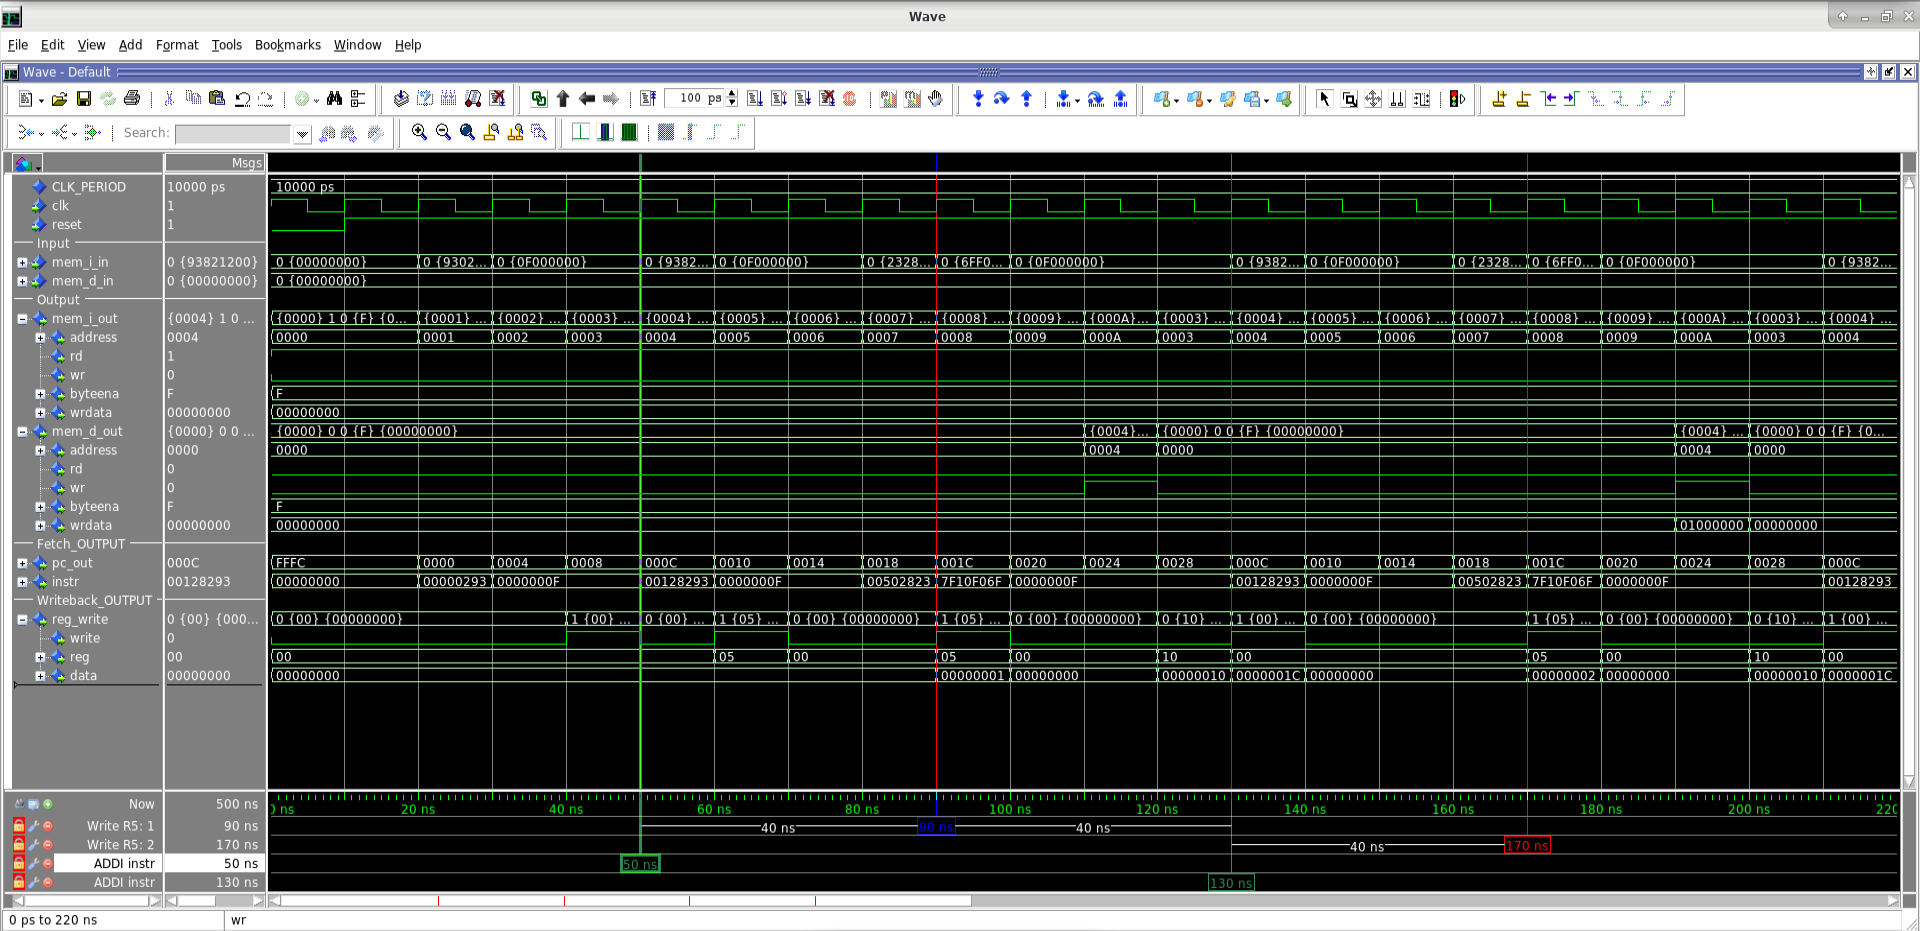
\includegraphics[width=1.0\linewidth]{pipeline.png}
  \caption{Simulation screenshot for Listing~\ref{lst:asmnofwd}.}
  \label{fig:sim}
\end{figure}

Make sure the following signals are visible in Figure~\ref{fig:sim} and the 
signal values are readable:
the program counter in the fetch stage, the instruction being fetched, the 
content of register \texttt{x5} and the fields \texttt{address}, \texttt{rd}, 
\texttt{wr}, \texttt{byteena}, and \texttt{wrdata} in the \texttt{mem\_out} 
signal coming out of the pipeline in the memory stage.

\begin{lstlisting}[language=,mathescape=false,float=ht,caption={Assembler example without forwarding},label=lst:asmnofwd]
        addi x5, x0, 0
        nop
        nop
loop:
        addi x5, x5, 1
        nop
        nop
        sw x5, 16(x0)
        jal x0, loop
        nop
        nop
        nop
\end{lstlisting}
%%%%%%%%%%%%%%%%%%%%%%%%%%%%%%%%%%%%%%%%%%%%%%%%%%%%%%%%%%%%%%%%%%%%%%%%%%%%%%%%
%%%%%%%%%%%%%%%%%%%%%%%%%%%%%%%%%%%%%%%%%%%%%%%%%%%%%%%%%%%%%%%%%%%%%%%%%%%%%%%%

\end{document}
